\documentclass[12pt,a4paper,titlepage,oneside]{report}
\usepackage[T1]{fontenc}
\usepackage{titlesec, blindtext, color}
\usepackage[spanish]{babel}
\usepackage[utf8]{inputenc}
\usepackage{lmodern}
\usepackage{graphicx}
\usepackage{subcaption}
\usepackage{pdfpages}
\usepackage{xcolor}
\usepackage{color}
\usepackage{url}
\usepackage{pdfpages}
\usepackage{fourier} % Use the Adobe Utopia font for the document - comment this line to return to the LaTeX default
\usepackage{amsmath,amsfonts,amsthm} % Math packages
\usepackage{listings}
\usepackage{caption}
\usepackage{titling}
\usepackage{lipsum} 
\usepackage{sectsty}
\usepackage{fancyhdr}
\usepackage{float}
\usepackage{tabulary}
\usepackage[colorlinks=true,linkcolor=black,urlcolor=blue,citecolor=black]{hyperref} 
\usepackage{booktabs}% http://ctan.org/pkg/booktabs
\usepackage{pgfplots}

\pagestyle{fancy}
\fancyhf{}
\fancyhead[LE,RO]{\nouppercase \leftmark}
\fancyhead[LO,RE]{\nouppercase \rightmark}
\fancyfoot[C]{\thepage}

\newcommand{\Keywords}[2]{\vfill\noindent{\small{\em Palabras clave}: }}
\newcommand{\KeywordsEn}[2]{\vfill\noindent{\small{\em KeyWords}: }}
\definecolor{grisclar}{gray}{0.5}
\definecolor{grisfosc}{gray}{0.25}

% Editar con los datos correspondientes
\newcommand{\titulo}{Controlador de riego de Cultivo Hidropónico}
\newcommand{\titulacion}{Master de Ingeniería Informática}
\newcommand{\autor}{}
%\newcommand{\director}{}

% Colors definitions

\definecolor{mygray}{rgb}{0.9,0.9,0.9} % Color definition
\definecolor{darkspringgreen}{rgb}{0.09, 0.45, 0.27}
\definecolor{babyblue}{rgb}{0.54, 0.81, 0.94}
\definecolor{airforceblue}{rgb}{0.36, 0.54, 0.66}
\definecolor{blue(ncs)}{rgb}{0.0, 0.53, 0.74}
\definecolor{gray75}{gray}{0.75}

\title{\titulo}
\author{\autor}
\renewcommand\chaptername{TFG}

\newcommand{\hsp}{\hspace{15pt}}
\titleformat{\chapter}[hang]{\Huge\bfseries}{\thechapter\hsp\textcolor{gray75}{|}\hsp}{0pt}{\Huge\bfseries}


%Comment -> Ctrl+T
%Uncomment -> Ctrl+U

\begin{document}
\begin{titlepage}
\begin{center}

\begin{minipage}{0.49\linewidth}
\begin{flushleft}

\includegraphics[height=1.5cm]{./images/logo_uhu}
\end{flushleft}
\end{minipage}
\begin{minipage}{0.49\linewidth}
\begin{flushright}

\includegraphics[height=1.5cm]{./images/logo_etsi}
\end{flushright}
\end{minipage}

\vspace{2cm}

\begin{color}{grisfosc}
\large
Escuela Técnica Superior de Ingeniería\\[0.2cm]
Universidad de Málaga\\[1.9cm]
\end{color}

% Título del proyecto y titulación
{\LARGE \bfseries \titulo}\\[1.5cm]
\textsc{\large Trabajo de prácticas}\\[0.4cm]
\textcolor{grisclar}{\large\titulacion}\\[5.0cm]

% Autor, director y fecha
\begin{flushright} \large
\emph{Autor:} \autor\\[0.4cm]
%\emph{Director:} \director\\[0.6cm]
\today
\end{flushright}

%\vfill
% Bottom of the page
%{\large \today}

\end{center}

\end{titlepage}


\lstset{ 
	  backgroundcolor=\color{white},
	  basicstyle=\footnotesize, 
	  breakatwhitespace=false, 
	  breaklines=true,     
	  captionpos=c,    
	  commentstyle=\color{darkspringgreen},
	  extendedchars=true,  
	  keepspaces=true,
	  keywordstyle=\color{blue},       % keyword style               
	  numbers=left,            
	  numbersep=7pt,  
	  rulecolor=\color{black},
	  showspaces=false,
	  showstringspaces=false,
	  showtabs=false,
	  stringstyle=\color{blue(ncs)},     % string literal style
	  tabsize=2	
}

\tableofcontents
\listoffigures

\chapter{Contexto y descripción}

	Dispositivo para controlar una estación de riego 
con múltiples salidas de riego. Dicho dispositivo 
permitirá controlar 1 boca de riego, con programación 
independiente, control de caudal en cada una de ellas, posibilidad 
de agrupar varias bocas, riego inteligente (según predicción/medición 
de lluvia, hora del día, sensor de humedad del suelo,...), arranque y
 parada de riego manual, avisos y estadísticas de riego. El conjunto del proyecto se plantea para que el cultivo sea hidropónico\footnote{El cultivo hidropónico es aquel que prescinde totalmente de la tierra para cultivar los alimentos.}

\section{Esquema básico del hardware}

	El esquema del proyecto se plantea de manera que sea necesario solo un dispositivo ESP8266 y una Raspberry Pi. El dispositivo Esp8266 se encargará de la lectura de los diferentes sensores junto a la actuación y decisión de activar los actuadores	correspondientes (Si es necesario cambiar el agua, activara la bomba pertinente).
	
	Como se muestra en la figura siguiente, se conectarán un sensor de humedad para comprobar el ambiente y en caso de necesidad se activará el motor de paso para proporcionar agua nueva o ventilar la estancia en caso de necesidad.
	
	\begin{figure}
		\center
		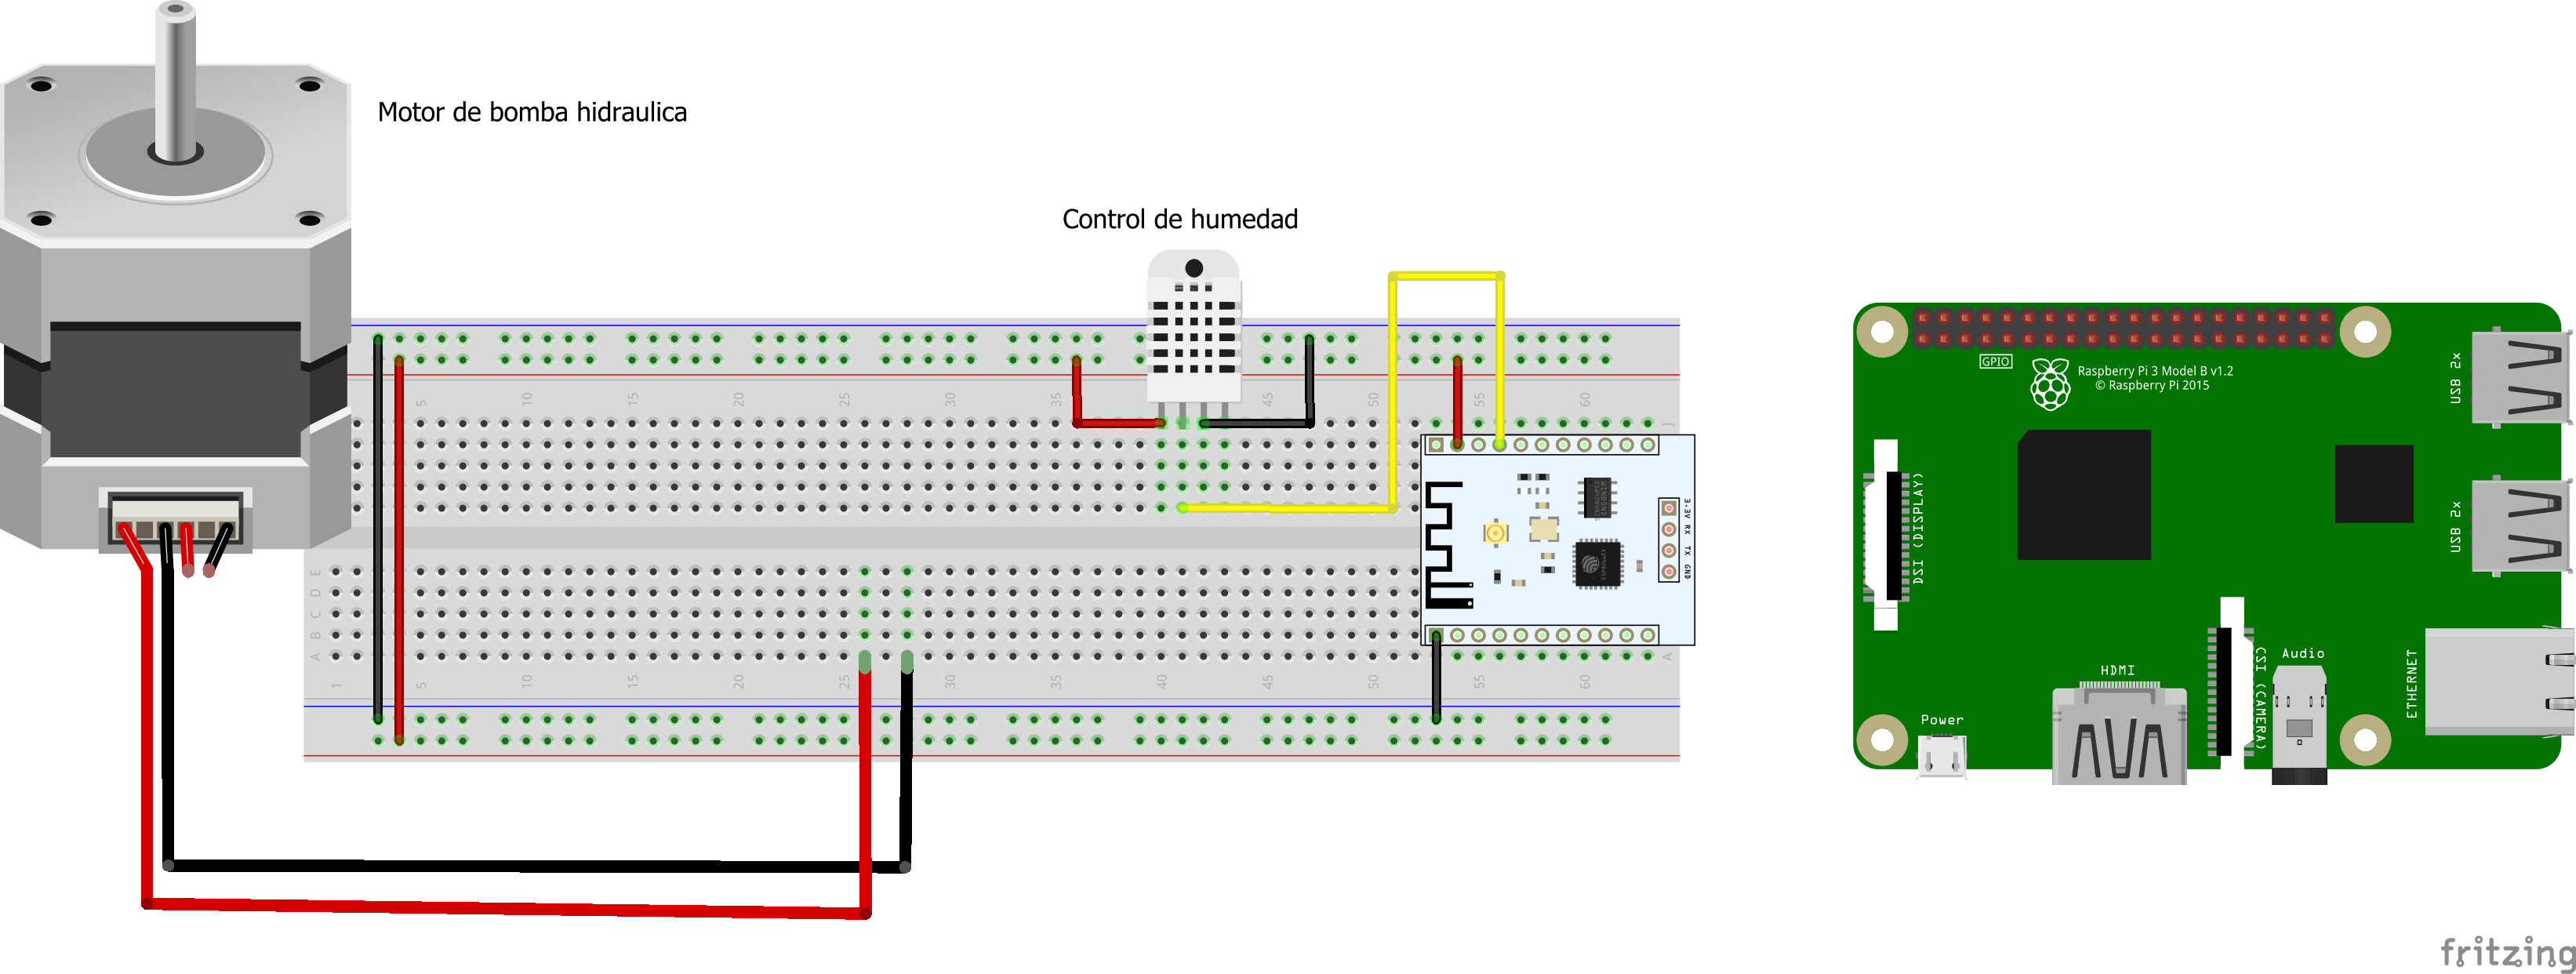
\includegraphics[scale=0.5]{./images/Conexion.png}
		\caption{Esquema básico de conexión Sensor-Sistema-Actuador}
		\label{Esquema_basico}
	\end{figure}		
	
	Para la realización se estima la utilización de los siguientes componentes:	
	
	\subsection*{Materiales varios}
	
		\begin{itemize}
			\item Tubos de plástico.	
			\item Recipiente donde almacenar el agua y controlar el pH de la misma.
			\item Bandeja donde colocar la planta y verter el agua.
			\item Canalización de plástico donde colocar la planta.
			\item Lana de roca.
			\item Recipientes tipo malla u otro recipiente que permita el paso del agua.
		\end{itemize}			
	
	\subsubsection*{Sensores}

		\begin{itemize}
			\item Humedad.
			\item Fotovoltaico.
			\item Temperatura.
			\item pH.
		\end{itemize}

	\subsubsection*{Actuadores}

		\begin{itemize}
			\item Bomba de riego.
			\item Motores de paso.
			\item Servo Motores.
			\item Interruptor (Encendido y apagado del sistema).
			\item ...
		\end{itemize}			
	
	\subsubsection*{Controladores}
		
		\begin{itemize}
			\item RaspberriPi.
			\item ESP8266 | NodemCu.
		\end{itemize}			
	
	\subsubsection*{Información a tratar}
		
		\begin{itemize}
			\item \textbf{Sensores-ESP8266:} los datos del cultivo que controla.
			\item \textbf{ESP8266-Actuadores:} diferentes ordenes para mantener el cultivo que controla.
			\item \textbf{ESP8266-RasPi:} los datos recogidos de los sensores.
			\item \textbf{RasPi-ESP8266:} Intrucciones correspondientes a los datos externos recogidos (Lluvia, temperatura, sol,...). Información del usuario | Internet.
			
		\end{itemize}

\chapter{Funcionamiento}

	El funcionamiento del proyecto consistirá en dos partes bien diferenciadas. La primera, está simbolizada en la figura siguiente \ref{Funcionamiento}, donde se irán leyendo los sensores cada cierto tiempo. En caso de necesidad se activarán los actuadores y en caso contrario el dispositivo quedará suspendido hasta que paso el tiempo correspondiente. También se activarán al principio de la ejecución la rutina de interrupción, para permitir qué, en el caso de que el dispositivo esté dormido y el usuario quiera realizar un cambio, se despierte y se realicen los cambios con los actuadores según ordene la placa Raspberry Pi.

	\begin{figure}
		\center
		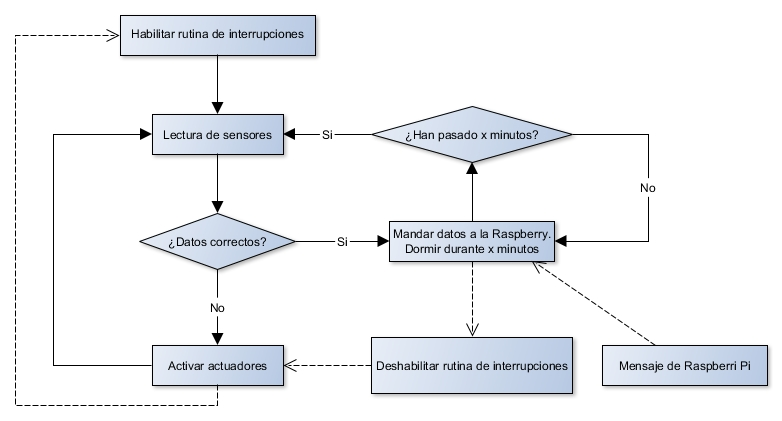
\includegraphics[scale=0.5]{./images/funcionamientoESP8266.jpg}
		\caption{Funcionamiento del módulo ESP8266}
		\label{Funcionamiento}
	\end{figure}
	
	La placa Raspberry, por el contrario, será la encargada de manejar la Base de Datos (BBDD) donde se almacenarán los datos recogidos por el Esp8266, y la interfaz gráfica con la que el usuario podrá interactuar con el sistema.

\chapter{ToDos}

	\subsection*{Programación de los diferentes componentes [Ok]}
	
	\subsection*{Preparación del cableado, junto con la posible soldadura requerida [Ok]}
	
	\subsection*{Construcción del modelo de jardinería donde instalar todos los componentes[-]}
	
	\subsection*{Instalación de los diferentes componentes en la jardinera [-]}
	
	\subsection*{Instalación de la BBDD MongoDB [Ok]}
	
	\subsection*{Programación de la BBDD [Ok]}
	
	\subsection*{Instalación de la API Node-Red [-]}
	
	\subsection*{Programación de la API con Node-Red [-]}
	
	\subsection*{Probar el sistema y solucionar posibles fallos [-]}

\chapter{Ampliaciones}

	\subsection*{Motor de control de persiana}
	
\end{document}
